\documentclass[tikz, border = 2pt]{standalone}

%---------------------------------------------------------------------------%
% PACKAGES                                                                  %
%---------------------------------------------------------------------------%

%----- MATH
%---------------------------------------------------------------------------%
\usepackage{amsmath, amssymb}
%----- FIGURES
%---------------------------------------------------------------------------%
\usepackage{pgfplots}
\pgfplotsset{compat=1.13}


\begin{document}

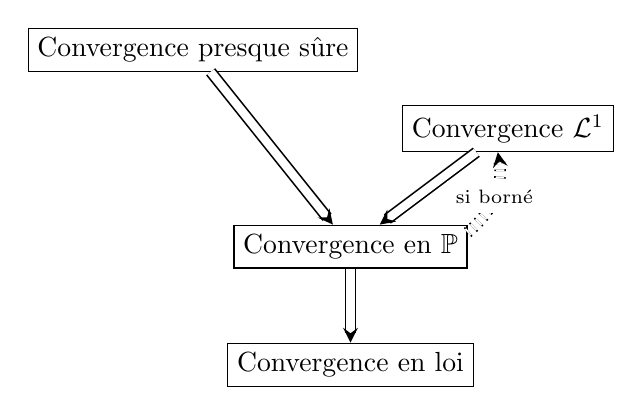
\begin{tikzpicture}
% définition des styles
\tikzstyle{quadri}=[rectangle,draw]
\tikzstyle{implique}=[->,double distance =3pt,>=stealth,semithick]
\tikzstyle{impliquecond}=[->,double distance =3pt,>=stealth,semithick,dotted]
% les nœuds
\node[quadri] (PS) at (0,0) {Convergence presque s\^ure};
\node[quadri] (M) at (4,-1) {Convergence $\mathcal{L}^1$};
\node[quadri] (P) at (2,-2.5) {Convergence en $\mathbb{P}$};
\node[quadri] (L) at (2,-4) {Convergence en loi};
% les flèches
\draw[implique] (PS)--(P);
\draw[implique] (M)--(P); 
\draw[implique] (P)--(L);
\draw[impliquecond] (P) to[bend right] node[midway,fill=white]{\scriptsize si born\'e} (M);
% la légende
\end{tikzpicture}

\end{document}